\subsection{Communication} \label{subsec:Communication}
The Main Processor and Sample Control modules need a communication interface in order to set control settings for the ADCs, DAC in the FPGA's internal registers and to retrieve stored ADC samples. The ADCs and DAC \todo{Vi mangler at redegøre for det her valg.} both have 16 bits of resolution and a 16 bit wide parallel bus between the FPGA and MCU will be used to transfer the data as shown on figure \refq{fig_7_2_1_CommBus}.

\begin{figure}[H]
    \centering
    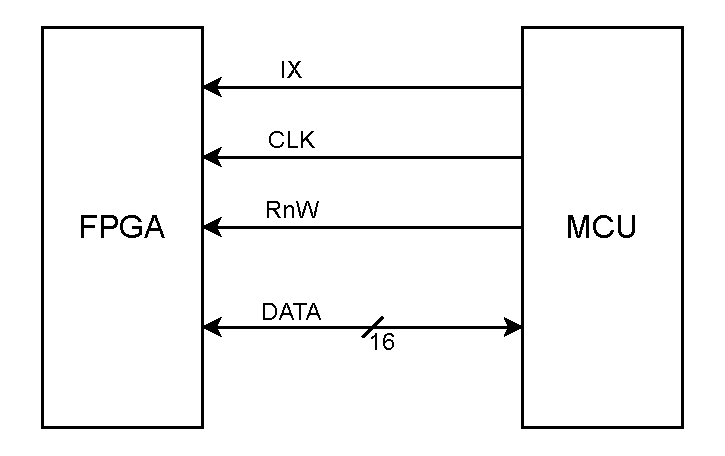
\includegraphics[clip, trim=0 0 0 0, width=0.6\textwidth]{Sections/7_SystemDesign/Figures/CommPort_Block.pdf}
    \caption{The communication bus connecting the FPGA and microcontroller. It uses a 16 bit databus, along with a CLK, a read/write control signal and Internal/External signal.}
    \label{fig_7_2_1_CommBus}
\end{figure}

The microcontroller is always going to be the master that has to initiate communication and the FPGA is always the slave. The microcontroller is controlling the read/write and CLK control signals necessary for the communication to work. The Read-write pin is, when  RW = '0', in write mode and in read mode when RW = '1'. Data is clocked in and out on the rising edges of the CLK. The IX pin is short for Internal/External and is used to tell the FPGA wheter the MCU wants to fetch data from the external sample memory or it wants to communicate with the internal registers of the FPGA. 

If the MCU wants to write some value into a register it must first CLK in an address into the FPGA before it can CLK in any data, as shown on figure \refq{fig_7_2_1_CommWrite}. Note that the external sample memory is read only for the MCU. When the MCU intends to commicate with the internal registers the IX pin is set to a logical '0', a '1' indicates that the MCU desires to fetch data from the external sample memory.
\begin{figure}[H]
    \centering
    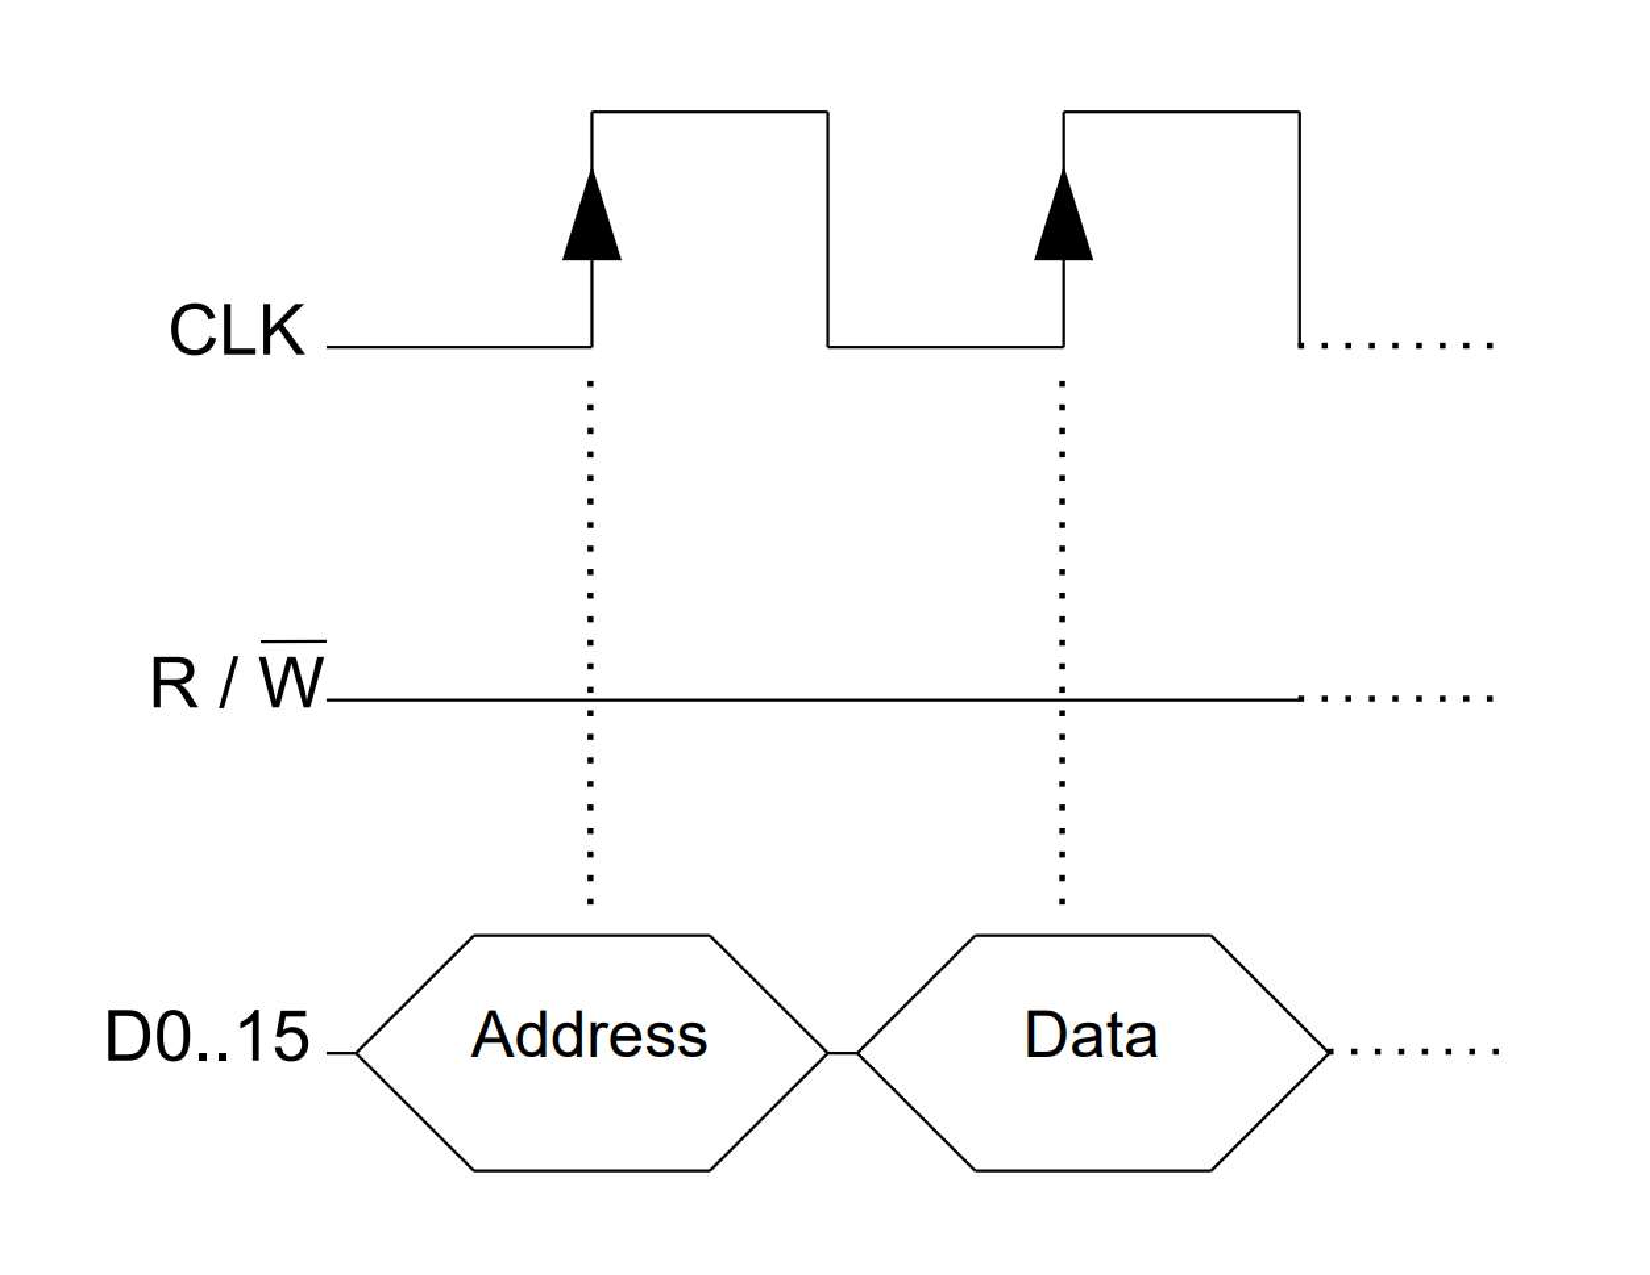
\includegraphics[clip, trim=0 45 0 0, width=0.5\textwidth]{Sections/7_SystemDesign/Figures/7_2_1_CommWrite.pdf}
    \caption{In order to write to the FPGA, the MCU must first set RW ='0' and IX = '0', (IX not shown) then set the 16 bit bus to the desired address and generate a single CLK pulse. The address is clocked into the FPGA on a rising edge. To write data into the address; the MCU sets 16 bit data on the bus and then generate a single clock pulse. Data is clocked into the FPGA on a rising edge.}
    \label{fig_7_2_1_CommWrite}
\end{figure}

Note how on figure \refq{fig_7_2_1_CommWrite} D0..D15 should have settled before the MCU tries to clock in any value. This will be ensured by design as the signals for the communication are generated sequentially in software on the MCU. They are not hardware controlled and there will be a minimum of \SIQ{35.8}{\nano\second} between D0..D15 and CLK as shown in appendix \refq{App:MicrocontrollerConsiderations} and significantly more if the MCU wants to read from the FPGA.

If the MCU wants to read from the FPGA, there are two ways to do so, i can read the internal register and the external sample memory. To read the internal reigsters the IX pin must be set to '0'. Hereafter it will clock in an address in write mode, then change it's D0..D15 output pins to input pins and set RW '1'. The following CLK will cause the FPGA to set the data unto the bus pins as shown on figure \refq{fig_7_2_1_CommRead} (IX not shown, as it is constantly '0' for this opperation). 

\begin{figure}[H]
    \centering
    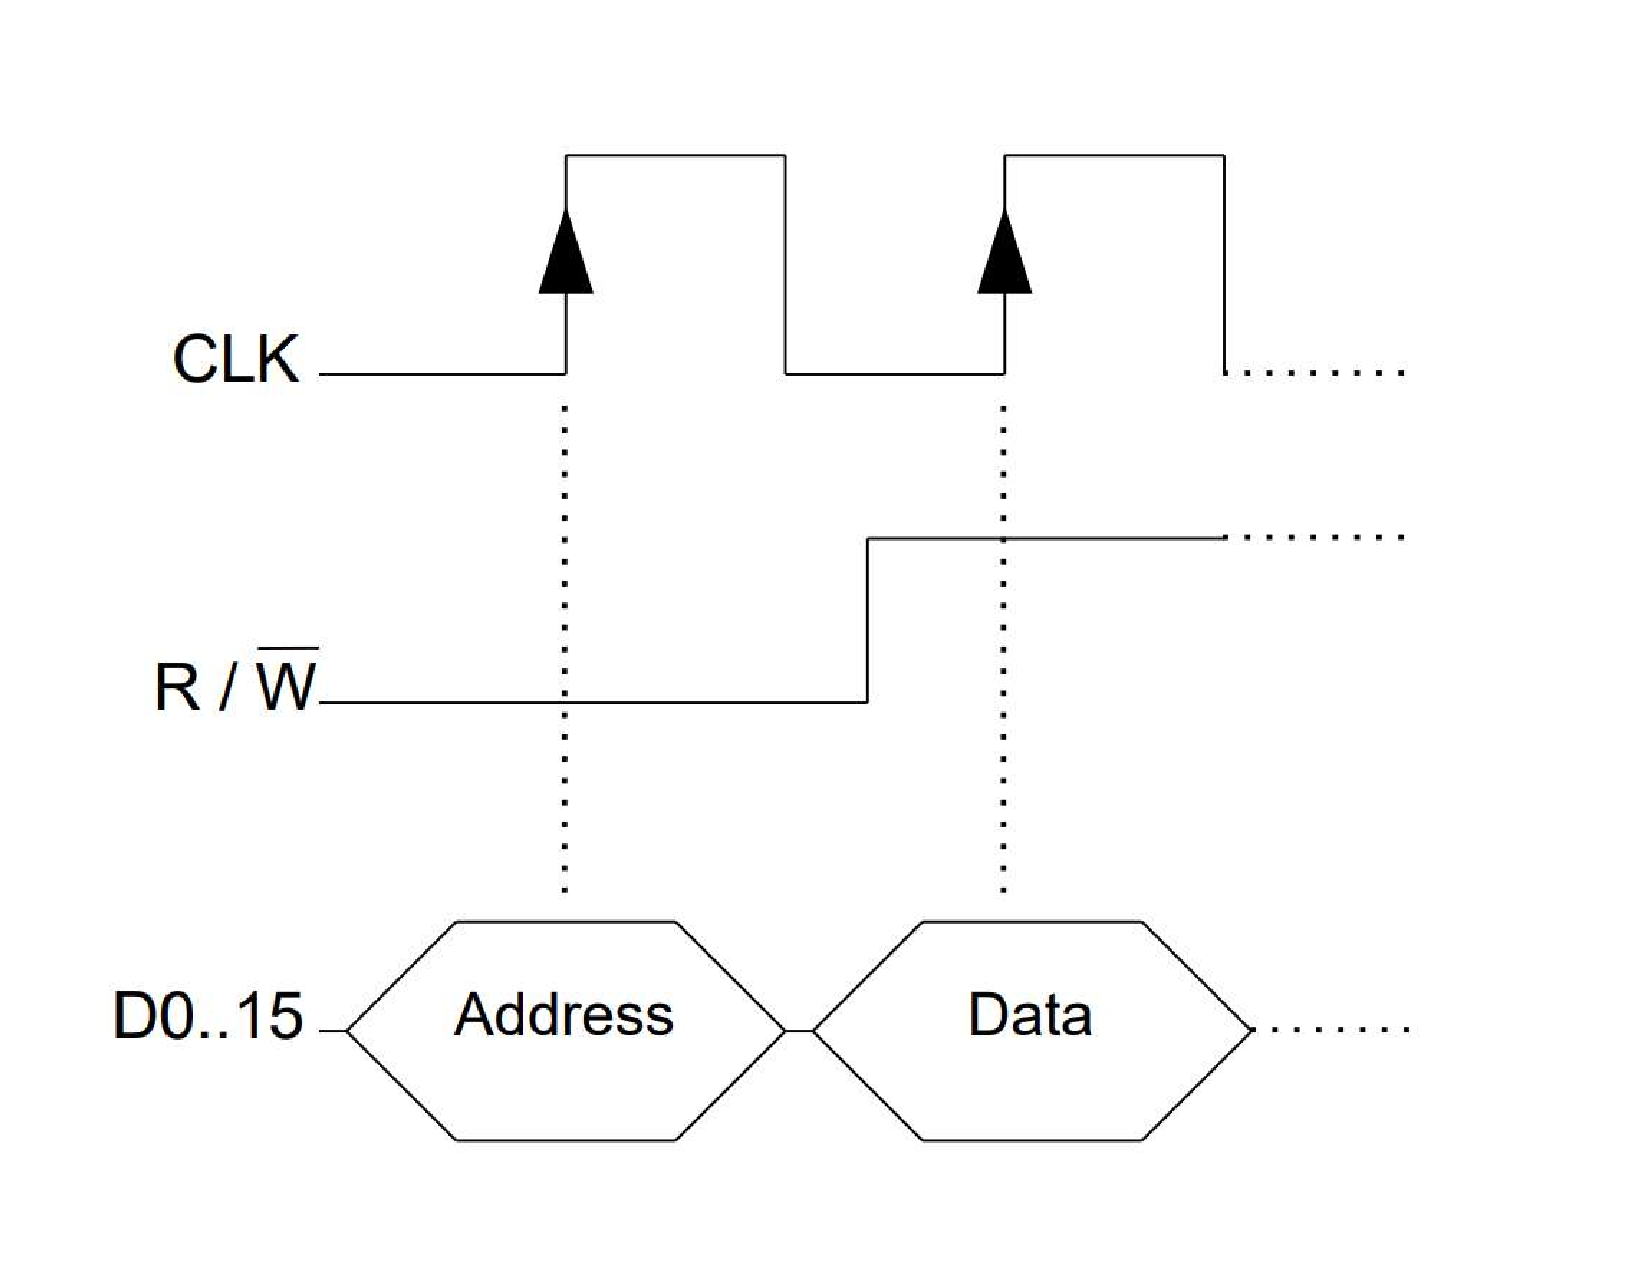
\includegraphics[clip, trim=0 50 0 0, width=0.5\textwidth]{Sections/7_SystemDesign/Figures/7_2_1_CommRead.pdf}
    \caption{In order to read from the FPGA sample memory, the MCU must first set RW ='0' then set the 16 bit bus to the desired address and generate a single CLK pulse. The address is clocked into the FPGA on a rising edge. To read data from the address; the MCU sets RW = '1' and changes it's DB0..DB15 outputs to inputs. The FPGA clocks the data out on DB0..DB15 on the next rising edge.}
    \label{fig_7_2_1_CommRead}
\end{figure}

Alternatively, if the MCU wishes to read from the external memory, its shall fist configure D0..D15 for inputs and then set IX and RW to '1'. Each rising edge of the clock will then clock out data from external memory, starting with address 0, each clock falling edge will then increase the address by one, such that the number of rising edges corresponds to the number of address that data has been fetched from. In this way, the MCU does not have to reconfigure its inputs, drastically increasing the rate of data-transfer and the goodput equals the throughput. The protocol for this can be seen in figure \ref{fig_7_2_1_CommRead_IX}. It should be noted that when a rising edge occurs on the clock, the FPGA uses about \SIQ{80}{\nano\second} to fetch the data, see section \ref{subsec:Sample_Memory_Distribution}. This means that the MCU must wait at least \SIQ{80}{\nano\second} before it stores the data on the port.

\begin{figure}[H]
    \centering
    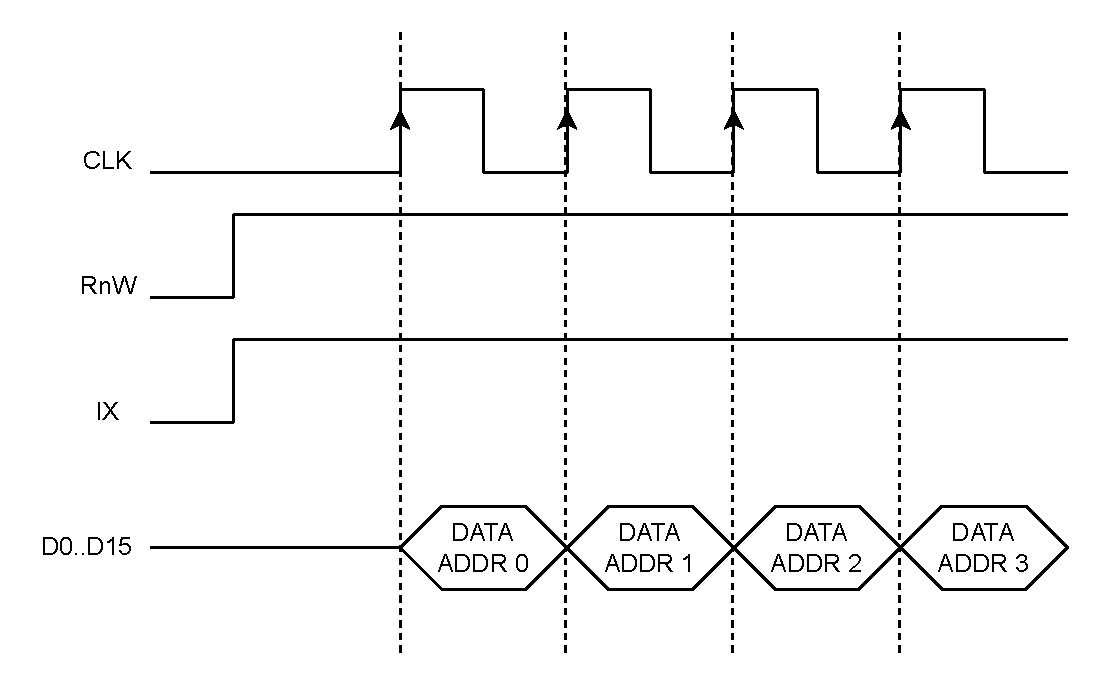
\includegraphics[clip, trim=0 0 0 0, width=0.8\textwidth]{Sections/7_SystemDesign/Figures/MCU_IX_FETCH.pdf}
    \caption{In order to read from the FPGAs external memory, the MCU must first configure the 16 bit bus as inputs, then set RW ='1' and IX = '1'. Each hereafter rising edge of the clock then clocks out data, starting at address 0 and counting up for each clock sent.}
    \label{fig_7_2_1_CommRead_IX}
\end{figure}

\subsubsection{IO Port}
The FPGA is using tri-state buffers to function as both inputs and outputs. The Artix 7 FPGA development board is an expensive component and it was decided to let the FPGA use open-drain outputs in order to reduce the risk of both FPGA and MCU actively driving the data bus because of a mistake during development. Xilinx offer a generic drag and drop INOUT port that can be tristated, this has been used. This IO buffer can be seen in figure \ref{fig_7_2_1_IOBUF} together with its truth table. Note that T acts inversly of what the RW pin does, T has simply been connected as not RW to fix this.

\begin{figure}[H]
    \centering
    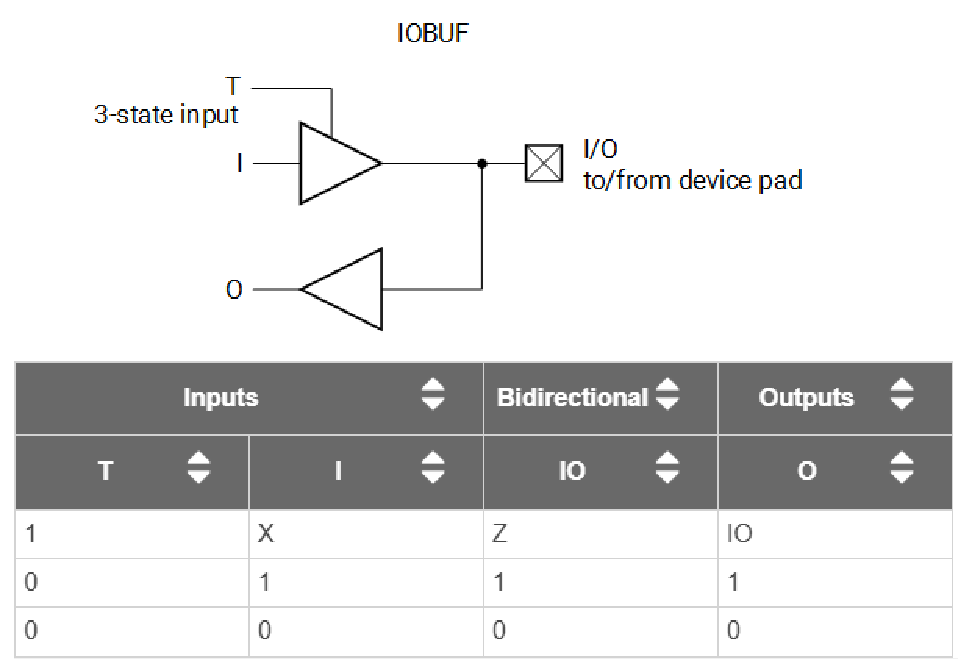
\includegraphics[clip, trim=0 0 0 0, width=0.7\textwidth]{Sections/7_SystemDesign/Figures/IOBUF.pdf}
    \caption{A truth table for the input/output port of the FPGA. T = '1' always puts the port into a high impedance state and T = '0' lets the port pull the I/O pin to '0', source: \cite{Xilinx_IOBUF}.}
    \label{fig_7_2_1_IOBUF}
\end{figure}

At first glance the I/O port logic on figure \refq{fig_7_2_1_IOBUF} may seem completely useless as it can't output a logic '1'. This is because the I/O pins will require external pull-up resistors in order to produce a '1' when T = '0'. This will reduce the chance of both FPGA and MCU driving the data bus at the same time. The only possible way of damaging the FPGA with the communication bus is if the MCU sets it's output high when T = '0' (RW = '1'), and the FPGA sets a '0' as the FPGA pins are high impedance in any other case.

\subsubsection{Communication data-rate} \label{subsubsec:CommunicationDatarate}

An estimate of the data-rate from this data bus can be made based on the findings in appendix \refq{App:MicrocontrollerConsiderations}. For consecutive read operations where the RW signal remains in 'write' mode, the data-rate will be limited by the execution time of setting the register in the STM32F446RE. This is also described in appendix \refq{App:MicrocontrollerConsiderations}. From the appendix it takes $t_{clk} = 35.8$ns to toggle the pin by setting and clearing a register and a write to a single register will take $t_{rs} = 17.9$ns. This is useful for calculating the communication throughput.

Every write operation to the RAM requires a 16bit address and 16bit data and two toggles of the CLK. It can be seen in appendix \refq{App:PinMap_MCU_FPGA} on the pin map that the data bus on the STM32F446Re is spread over two separate ports, so the MCU will have to write(and read) to two separate registers in order to write to the FPGA. This is a limitation of the Nucleo development board being used, it would otherwise be possible to do this with a single port, and thus a single register transfer. The total amount of register writes for a single write operation will be as shown in eq \refq{eq:7_2_1_Write_ThroughPut}.

\begin{equation}\label{eq:7_2_1_Write_ThroughPut}
    n_{reg} = n_{clk} +  n_{address} + n_{write} = 4+2+2 = 8 
\end{equation}
It takes a total of 8 register writes to perform a single write operation to the FPGA as shown in equation \refq{eq:7_2_1_Write_ThroughPut}. 4 for toggling the CLK pin twice and 2 each for setting the address and data on the IO pins. Each register write takes \SIQ{17.9}{\nano\second} so the total execution times for a write operation is \SIQ{143.2}{\nano\second} as shown in eq\refq{eq:7_2_1_Write_ThroughPutTotalTime}.
\begin{equation}\label{eq:7_2_1_Write_ThroughPutTotalTime}
    t_{write} = t_{rs} \cdot n_{reg} = 17.9e-9 \cdot 8 =  143.2e-9
\end{equation}
It takes \SIQ{143.2}{\nano\second} for the MCU to perform a write operation. The total throughput on the bus in write mode will be about \SIQ{7}{\mega\bit}/s as shown in equation \refq{eq:7_2_1_Write_ThroughPut}.

\begin{equation}\label{eq:7_2_1_Write_ThroughPut}
    R_{write} = \frac{1}{t_{write}} = 6.949e6 
\end{equation}
The throughput on the bus is about \SIQ{7}{\mega\bit}/s in write mode. A significant amount of the throughput is used on protocol overhead as half the transmissions are addresses. The protocol efficiency is thus $\eta_{write} = 0.5$. The goodput will be as in eq \refq{eq:7_2_1_Write_ThroughPut2}.
\begin{equation}\label{eq:7_2_1_Write_ThroughPut2}
    G_{write} = R_{write}\cdot \eta_{write} = 6.949e6 \cdot 0.5 = 3.475e6 
\end{equation}
The goodput of the bus in write mode is \SIQ{3.475}{\mega\bit}/s for consecutive writes. The situation is different for consecutive MCU read operations as it will have to toggle it's GPIO modes from output to input in each read operation. It takes $t_{mode} = 181.2$ns to toggle between GPIO input and output modes as found in appendix \refq{App:MicrocontrollerConsiderations}. For a consecutive read operation when the MCU reads internal registers, the MCU will have to perform two of these transitions. The MCU will also need to toggle the RW pin along with, those are two register operations and it will have to set an address on the GPIO pins. The total amount of transitions is shown in eq \refq{eq:7_2_1_Read_Register1}.

\begin{equation}\label{eq:7_2_1_Read_Register1}
    n_{read} = n_{clk} + n_{address} + n_{RW} + {n_mode} = 5 \cdot n_{rs} + 2 \cdot n_{mode} 
\end{equation}

The total time for a read operation will thus be $t_{read} = 451.9$ns as shown in eq \refq{eq:7_2_1_Read_Register2}.
\begin{equation}\label{eq:7_2_1_Read_Register2}
    t_{read} = 5\cdot 17.9e-9 + 2\cdot 181.2e-9 = 451.9e-9 
\end{equation}
The throughput of the data bus for consecutive read modes will be \SIQ{2.213}{\mega\bit}/s as shown in equation \refq{eq:7_2_1_Read_Throughput}.
\begin{equation}\label{eq:7_2_1_Read_Throughput}
    R_{read} = \frac{1}{t_{read}} =\frac{1}{451.9e-9} = 2.213e6  
\end{equation}
Once again, the address is 'wasted' data and the goodput on the bus will be halved by $\eta_{read} = 0.5$, so the goodput on the bus is about \SIQ{1.1}{\mega\bit}/s as shown in eq \refq{eq:7_2_1_Read_Goodput}.
\begin{equation}\label{eq:7_2_1_Read_Goodput}
    G_{read} = \eta_{read} \cdot  = 2.213e6\cdot 0.5  = 1.106e6 
\end{equation}
To increase the data-rate when sample data is to be fetched, the IX pin was introduced, this removes the need for the MCU to reconfigure its outputs altogether. This means that the MCU needs to sent a clock, wait \SIQ{100}{\nano\second} to allow the FPGA to get the data, and then read the data on the bus. An estimate of the data-rate when reading samples can thus be made by looking at the total amount of register commands needed to send a clock and read the IO port. This can be seen in equation \ref{eq:7_2_1_SampleReadReg}.
\begin{equation}\label{eq:7_2_1_SampleReadReg}
    n_{reg-sample} = n_{clk}+n_{read} = 2+2 = 4
\end{equation}

An estimate of how much time it takes to read a single sample data register can then be made, where the \SIQ{100}{\nano\second} time used by the FPGA is added. This is found the be \SIQ{172}{\nano\second}, see equation \ref{eq:7_2_1_SampleReadTime}.

\begin{equation}\label{eq:7_2_1_SampleReadTime}
    t_{sample} = n_{reg-sample}*17.9E-9 + 100e-9 = 4*17.9e-9+100e-9 = 171.6e-9
\end{equation}

Finally it can be estimated that the time required to fetch data from all 10000 samples (20000 registers due to current and voltage being sampled) is $20000\cdot171.6e-9 = \SIQ{3.43}{\milli\second}$ with 100\% efficiency. This is however rather optimistic, as the FPGA is not actively driving the output, but pull-up resistors are, greatly increasing the rise time. Rough measurements with internal pull-up resistors have shown a rise time of about \SIQ{800}{\nano\second}. Taking this in to the equation yields the single register read time as seen in equation \ref{eq:7_2_1_SampleReadTimeWrise}. This results in a more realistic estimate of $20000\cdot 971.6e-6 = \SIQ{19.4}{\milli\second}$. This can however be improved by the use of external pull-up resistors.

\begin{equation}\label{eq:7_2_1_SampleReadTimeWrise}
    \begin{split}
        t_{sample} = &n_{reg-sample}*17.9E-9 + 100e-9+t_{rise} \\
        \Rightarrow t_{sample} = &4*17.9e-9+100e-9+800e-9 = 971.6e-9
    \end{split}
\end{equation}
